% !TEX program = xelatex
\documentclass[UTF8]{ctexart}

\RequirePackage{inputenc}
\RequirePackage{fontspec}
\RequirePackage{xeCJK}

\RequirePackage{amsmath}
\RequirePackage{amssymb}
\RequirePackage{mathpazo}
\RequirePackage{pgfplots}
\RequirePackage{tikz}
\RequirePackage{tkz-euclide}

\usetkzobj{all}

\RequirePackage{subfigure}

\setmainfont{Times New Roman}

\setCJKmainfont{等线}
\setCJKsansfont{等线}
\setCJKmonofont{等线}

\let\nvec\vec
\def\vec#1{\nvec{\vphantom b\smash{#1}}}

\newcommand*{\dif}{\mathop{}\!\mathrm{d}}

\renewcommand{\Re}{\operatorname{Re}}
\renewcommand{\Im}{\operatorname{Im}}
\newcommand{\arccot}{\operatorname{arccot}}

\makeatletter
\newcommand{\rmnum}[1]{\romannumeral #1}
\newcommand{\Rmnum}[1]{\expandafter\@slowromancap\romannumeral #1@}
\makeatother

\usepackage{geometry}
\geometry
{
    left=1.25in,
    right=1.25in,
    top=1in,
    bottom=1in
}

\title{数学扩展研究\Rmnum{1}~~-~~三角形}
\author{李宇轩}
\date{2020.03.09}

\begin{document}

\maketitle

\newpage

\tableofcontents

\newpage

\setlength{\parindent}{0pt}

\section{三角形}

\subsection{三角形的符号约定}
    我们首先进行符号约定,若没有特殊说明,这些符号将在后文表达相同的含义。\\[3mm]
    我们依照下方表格的规定进行符号约定:\vspace{5pt}
    \begin{table}[h]
        \begin{center}
            \begin{tabular}{l|l|l|l}
                \hline
                符号~~~~~~~~&含义~~~~~~~~~~~~~~~~~~~~~~~~~~~~~~~~~~~~~~~~~~~~&符号~~~~~~~~&含义~~~~~~~~~~~~~~~~~~~~~~~~~~~~~~~~~~~~~~~~~~~~\\ \hline
                $A$&角$A$的角度&$h_a$&垂线的长度(边$a$上)\\ \hline
                $B$&角$B$的角度&$h_b$&垂线的长度(边$b$上)\\ \hline
                $C$&角$C$的角度&$h_c$&垂线的长度(边$c$上)\\ \hline
                $a$&边$a$的长度&$m_a$&中线的长度(边$a$上)\\ \hline
                $b$&边$b$的长度&$m_b$&中线的长度(边$b$上)\\ \hline
                $c$&边$c$的长度&$m_c$&中线的长度(边$c$上)\\ \hline
                $R$&外接圆半径&$t_a$&角平分线的长度(角$a$上)\\ \hline
                $r$&内切圆半径&$t_b$&角平分线的长度(角$b$上)\\ \hline
                $r_a$&旁切圆半径(边$a$侧)&$t_c$&角平分线的长度(角$c$上)\\ \hline
                $r_b$&旁切圆半径(边$b$侧)&$p$&半周长的大小\\ \hline
                $r_c$&旁切圆半径(边$c$侧)&&\\ \hline
            \end{tabular}
            \caption{三角形的符号约定}
        \end{center}
    \end{table}\\
    我们将下方图片所示的三角形作为参考:
    \begin{figure}[h]
        \begin{center}
            \begin{tikzpicture}
                \tkzInit[xmin=-0.5,xmax=8,ymin=-0.5,ymax=5]
                \tkzClip
                \tkzDefPoint(6,4.5){A}
                \tkzDefPoint(0,0){B}
                \tkzDefPoint(7.5,0){C}
                \tkzLabelPoints[above](A)
                \tkzLabelPoints[left](B)
                \tkzLabelPoints[right](C)
                \tkzDrawSegments(A,B)
                \tkzDrawSegments(B,C)
                \tkzDrawSegments(C,A)

                \tkzDefMidPoint(B,C) \tkzGetPoint{a}
                \tkzDefMidPoint(C,A) \tkzGetPoint{b}
                \tkzDefMidPoint(A,B) \tkzGetPoint{c}

                \tkzLabelPoints[below](a)
                \tkzLabelPoints[right](b)
                \tkzLabelPoints[above](c)
            \end{tikzpicture}
            \caption{三角形的示意图}
        \end{center}
    \end{figure}\\
    除此之外,重心记为$G$,垂心记为$H$,外心记为$O$,内心记为$I$,旁心记为$P$。

\newpage

\subsection{三角形的第一组面积公式}
    本章将研究三角形中较为基本的面积公式,并进行相应推导。

\subsubsection{三角形面积公式$01$}
    三角形面积公式$01$:
    \begin{large}
        \begin{align*}
            S_{\triangle}=\frac{1}{2}\cdot a\cdot h_a\\[2mm]
            S_{\triangle}=\frac{1}{2}\cdot b\cdot h_b\\[2mm]
            S_{\triangle}=\frac{1}{2}\cdot b\cdot h_b
        \end{align*}
    \end{large}\vspace{-20pt}

\subsubsection{三角形面积公式$02$}
    三角形面积公式$02$:
    \begin{large}
        \begin{align*}
            S_{\triangle}=\frac{1}{2}\cdot a\cdot b\cdot\sin{C}\\[2mm]
            S_{\triangle}=\frac{1}{2}\cdot b\cdot c\cdot\sin{A}\\[2mm]
            S_{\triangle}=\frac{1}{2}\cdot c\cdot a\cdot\sin{B}
        \end{align*}
    \end{large}\\
    将高用边和角的正弦表示并代入公式$01$:\vspace{5pt}
    \setcounter{equation}{0}
    \begin{align}
        S_{\triangle}
        &=\frac{1}{2}\cdot a\cdot h_a\\[3mm]
        &=\frac{1}{2}\cdot a\cdot (b\cdot \sin{C})
    \end{align}
    \begin{figure}[h!]
        \begin{center}
            \begin{tikzpicture}
                \tkzInit[xmin=-0.5,xmax=5.5,ymin=-0.5,ymax=3.5]
                \tkzClip
                \tkzDefPoint(4,3){A}
                \tkzDefPoint(0,0){B}
                \tkzDefPoint(5,0){C}
                \tkzLabelPoints[above](A)
                \tkzLabelPoints[left](B)
                \tkzLabelPoints[right](C)
                
                \tkzDrawSegments(A,B)
                \tkzDrawSegments(B,C)
                \tkzDrawSegments(C,A)

                \tkzDefMidPoint(B,C) \tkzGetPoint{a}
                \tkzDefMidPoint(C,A) \tkzGetPoint{b}
                \tkzDefMidPoint(A,B) \tkzGetPoint{c}

                \tkzDefLine[orthogonal=through A](B,C)
                \tkzGetPoint{a}
                \tkzInterLL(A,a)(B,C)
                \tkzGetPoint{D}

                \tkzDefLine[orthogonal=through B](C,A)
                \tkzGetPoint{b}
                \tkzInterLL(B,b)(C,A)
                \tkzGetPoint{E}

                \tkzDefLine[orthogonal=through C](A,B)
                \tkzGetPoint{c}
                \tkzInterLL(C,c)(A,B)
                \tkzGetPoint{F}

                \tkzDrawSegments(A,D)
                \tkzDrawSegments(B,E)
                \tkzDrawSegments(C,F)

                \tkzMarkRightAngle[scale=0.5](A,D,B)
                \tkzMarkRightAngle[scale=0.5](B,E,C)
                \tkzMarkRightAngle[scale=0.5](C,F,B)

            \end{tikzpicture}
            \caption{三角形面积公式$02$示意图}
        \end{center}
    \end{figure}

\newpage

\subsubsection{三角形面积公式$03$}
    三角形面积公式$03$:
    \begin{large}
        \begin{equation*}
            S_{\triangle}=\frac{1}{4R}\cdot a\cdot b\cdot c
        \end{equation*}
    \end{large}\\
    将正弦定理代入公式$02$:
    \setcounter{equation}{0}
    \begin{align}
        S_{\triangle}
        &=\frac{1}{2}\cdot a\cdot b\cdot\sin{C}\\[3mm]
        &=\frac{1}{2}\cdot a\cdot b\cdot\left(\frac{c}{2R}\right)\\[3mm]
        &=\frac{1}{4R}\cdot a\cdot b\cdot c
    \end{align}\\[2mm]

\subsubsection{三角形面积公式$04$}
    三角形面积公式$04$:
    \begin{large}
        \begin{equation*}
            S_{\triangle}=2R^2\cdot\sin{A}\cdot\sin{B}\cdot\sin{C}
        \end{equation*}
    \end{large}\\
    将正弦定理代入公式$02$:
    \begin{align}
        S_{\triangle}
        &=\frac{1}{2}\cdot  a\cdot b\cdot\sin{C}\\[3mm]
        &=\frac{1}{2}\cdot(2R\cdot\sin{A})\cdot(2R\cdot\sin{B})\cdot\sin{C}\\[3mm]
        &=2R^2\cdot\sin{A}\cdot\sin{B}\cdot\sin{C}
    \end{align}

\newpage

\subsubsection{三角形面积公式$05$}
    三角形面积公式$05$:
    \begin{large}
        \begin{equation*}
            S_{\triangle}=r\cdot p
        \end{equation*}
    \end{large}\\
    用角平分线将三角形分为三个小三角形:
    \setcounter{equation}{0}
    \begin{align}
        S_{\triangle}
        &=S_{\triangle IBC}+S_{\triangle ICA}+S_{\triangle IAB}\\[3mm]
        &=\frac{1}{2}\cdot a\cdot r+\frac{1}{2}\cdot b\cdot r+\frac{1}{2}\cdot c\cdot r\\[3mm]
        &=\frac{1}{2}\cdot(a+b+c)\cdot r\\[3mm]
        &=r\cdot p
    \end{align}
    \begin{figure}[htbp]
        \begin{center}
            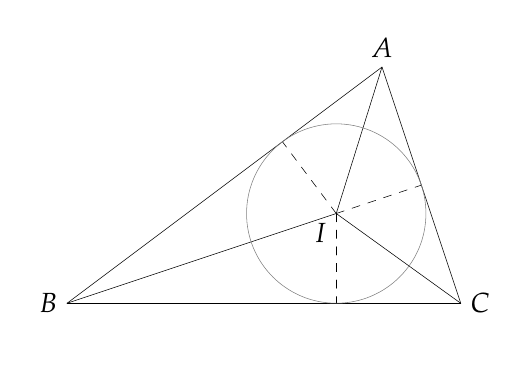
\begin{tikzpicture}
                \tkzInit[xmin=-0.5,xmax=5.5,ymin=-0.5,ymax=3.5]
                \tkzClip
                \tkzDefPoint(4,3){A}
                \tkzDefPoint(0,0){B}
                \tkzDefPoint(5,0){C}
                \tkzLabelPoints[above](A)
                \tkzLabelPoints[left](B)
                \tkzLabelPoints[right](C)
                \tkzDrawSegments(A,B B,C C,A)
            
                \tkzDefCircle[in](A,B,C)
                \tkzGetPoint{I}
                \tkzLabelPoints[below left](I)
            
                \tkzDrawSegments(A,I);
                \tkzDrawSegments(B,I);
                \tkzDrawSegments(C,I);
            
                \tkzDefLine[orthogonal=through I](A,B)
                \tkzGetPoint{r1}
                \tkzInterLL(I,r1)(A,B)
                \tkzGetPoint{R1}

                \tkzDefLine[orthogonal=through I](B,C)
                \tkzGetPoint{r2}
                \tkzInterLL(I,r2)(B,C)
                \tkzGetPoint{R2}

                \tkzDefLine[orthogonal=through I](C,A)
                \tkzGetPoint{r3}
                \tkzInterLL(I,r3)(C,A)
                \tkzGetPoint{R3}

                \tkzDrawSegments[dashed](I,R1)
                \tkzDrawSegments[dashed](I,R2)
                \tkzDrawSegments[dashed](I,R3)

                \tkzDrawCircle(I,R1)

            \end{tikzpicture}
            \caption{三角形面积公式$05$示意图}
        \end{center}
    \end{figure}

\newpage

\subsubsection{三角形面积公式$06$}
    三角形面积公式$06$:
    \begin{large}
        \begin{equation*}
            S_{\triangle}=r^2\cdot\left(\cot{\frac{A}{2}}+\cot{\frac{B}{2}}+\cot{\frac{C}{2}}\right)
        \end{equation*}
    \end{large}\\
    将边长用内切圆半径和角的余切表示并代入公式$05$:
    \begin{align}
        S_{\triangle}
        &=r\cdot p\\[3mm]
        &=r\cdot\frac{1}{2}\cdot(a+b+c)\\[3mm]
        &=r\cdot\frac{1}{2}\cdot\left(2r\cdot\cot{\frac{A}{2}}+2r\cdot\cot{\frac{B}{2}}+2r\cdot\cot{\frac{C}{2}}\right)\\[3mm]
        &=r^2\cdot\left(\cot{\frac{A}{2}}+\cot{\frac{B}{2}}+\cot{\frac{C}{2}}\right)
    \end{align}\\

\subsubsection{三角形面积公式$07$}
    三角形面积公式$07$:
    \begin{large}
        \begin{equation*}
            S_{\triangle}=R\cdot r\cdot(\sin{A}+\sin{B}+\sin{C})
        \end{equation*}
    \end{large}\\
    将正弦定理代入公式$05$:
    \setcounter{equation}{0}
    \begin{align}
        S_{\triangle}
        &=r\cdot p\\[3mm]
        &=r\cdot\frac{1}{2}\cdot(a+b+c)\\[3mm]
        &=r\cdot\frac{1}{2}\cdot(2R\cdot\sin{A}+2R\cdot\sin{B}+2R\cdot\sin{C})\\[3mm]
        &=R\cdot r\cdot(\sin{A}+\sin{B}+\sin{C})
    \end{align}

\newpage

\subsubsection{三角形面积公式$08$}
    三角形面积公式$08$:
    \begin{large}
        \begin{align*}
            S_{\triangle}=\frac{1}{2}\cdot\sqrt{~a^2\cdot b^2-\left(\frac{a^2+b^2-c^2}{2}\right)^2}\\[4mm]
            S_{\triangle}=\frac{1}{2}\cdot\sqrt{~b^2\cdot c^2-\left(\frac{b^2+c^2-a^2}{2}\right)^2}\\[4mm]
            S_{\triangle}=\frac{1}{2}\cdot\sqrt{~c^2\cdot a^2-\left(\frac{c^2+a^2-b^2}{2}\right)^2}
        \end{align*}
    \end{large}\\
    对公式$02$进行变形:
    \setcounter{equation}{0}
    \begin{align}
        S_{\triangle}
        &=\frac{1}{2}\cdot a\cdot b\cdot\sin{C}\\[3mm]
        &=\frac{1}{2}\cdot a\cdot b\cdot\sqrt{1-\cos^2{C}}\\[3mm]
    \end{align}\\
    将余弦定理代入:
    \begin{align}
        S_{\triangle}
        &=\frac{1}{2}\cdot a\cdot b\cdot\sqrt{1-\left(\frac{a^2+b^2-c^2}{2\cdot a\cdot b}\right)}\\[3mm]
        &=\frac{1}{2}\cdot\sqrt{a^2\cdot b^2 -\left(\frac{a^2+b^2-c^2}{2}\right)}
    \end{align}\\
    三角形面积公式$08$也被称为秦九韶公式。

\newpage

\subsubsection{三角形面积公式$09$}
    三角形面积公式$09$:
    \begin{large}
        \begin{equation*}
            S_{\triangle}=\sqrt{p\cdot(p-a)\cdot(p-b)\cdot(p-c)}
        \end{equation*}
    \end{large}\\
    对公式$02$进行变形:
    \setcounter{equation}{0}
    \begin{align}
        S_{\triangle}
        &=\frac{1}{2}\cdot a\cdot b\cdot\sin{C}\\[3mm]
        &=\sqrt{\left(\frac{a\cdot b}{2}\right)^2\cdot\sin^2{C}}\\[3mm]
        &=\sqrt{\left(\frac{a\cdot b}{2}\right)^2\cdot\left(1-\cos^2{C}\right)}\\[3mm]
        &=\sqrt{\left(\frac{a\cdot b}{2}\right)^2\cdot(1+\cos{C})\cdot(1-\cos{C})}\\[3mm]
        &=\sqrt{\frac{a\cdot b\cdot(1+\cos{C})}{2}\cdot\frac{a\cdot b\cdot(1-\cos{C})}{2}}
    \end{align}\\
    将余弦定理代入:
    \begin{align}
        S_{\triangle}
        &=\sqrt{\frac{a\cdot b\cdot\left(1+\dfrac{a^2+b^2-c^2}{2\cdot a\cdot b}\right)}{2}\cdot\frac{a\cdot b\cdot\left(1-\dfrac{a^2+b^2-c^2}{2\cdot a\cdot b}\right)}{2}}\\[3mm]
        &=\sqrt{\frac{a\cdot b+\dfrac{a^2+b^2-c^2}{2}}{2}\cdot\frac{a\cdot b-\dfrac{a^2+b^2-c^2}{2}}{2}}\\[3mm]
        &=\sqrt{\frac{\left(a^2+2ab+b^2\right)-c^2}{4}\cdot\frac{c^2-\left(a^2-2ab+b^2\right)}{4}}\\[3mm]
        &=\sqrt{\frac{\left(a+b\right)^2-c^2}{4}\cdot\frac{c^2-\left(a+b\right)^2}{4}}\\[3mm]
        &=\sqrt{\frac{a+b+c}{2}\cdot\frac{a+b-c}{2}\cdot\frac{c+a-b}{2}\cdot\frac{c-a+b}{2}}\\[3mm]
        &=\sqrt{p\cdot(p-a)\cdot(p-b)\cdot(p-c)}
    \end{align}\\
    三角形面积公式$09$也被称为海伦公式。

\newpage

\subsubsection{三角形面积公式$10$}
    三角形面积公式$10$:
    \begin{large}
        \begin{align*}
            &S_{\triangle}=\frac{1}{4}\cdot\sqrt{\left[(a+b)^2-c^2\right]\cdot\left[c^2-(a+b)^2\right]}\\[3mm]
            &S_{\triangle}=\frac{1}{4}\cdot\sqrt{\left[(b+c)^2-a^2\right]\cdot\left[a^2-(b+c)^2\right]}\\[3mm]
            &S_{\triangle}=\frac{1}{4}\cdot\sqrt{\left[(c+a)^2-b^2\right]\cdot\left[b^2-(c+a)^2\right]}
        \end{align*}
    \end{large}\\
    对公式$08$进行变形:
    \setcounter{equation}{0}
    \begin{large}
        \begin{align}
            S_{\triangle}
            &=\frac{1}{2}\cdot\sqrt{a^2\cdot b^2-\left(\frac{a^2+b^2-c^2}{2}\right)^2}\\[4mm]
            &=\frac{1}{2}\cdot\sqrt{\left(a\cdot b+\frac{a^2+b^2-c^2}{2}\right)\cdot\left(a\cdot b-\frac{a^2+b^2-c^2}{2}\right)}\\[4mm]
            &=\frac{1}{4}\cdot\sqrt{\left(a^2+b^2+2ab-c^2\right)\cdot\left(c^2-a^2-b^2+2ab\right)}\\[4mm]
            &=\frac{1}{4}\cdot\sqrt{\left[(a+b)^2-c^2\right]\cdot\left[c^2-(a-b)^2\right]}
        \end{align}
    \end{large}\\
    三角形面积公式$10$常用于解决已知三角形边长和与边长差的问题。

\newpage

\subsubsection{三角形面积公式$11$}
    三角形面积公式$11$:
    \begin{large}
        \begin{align*}
            S_{\triangle}=h_a~^2\cdot\frac{\sin{A}}{2\cdot\sin{B}\cdot\sin{C}}\\[3mm]
            S_{\triangle}=h_b~^2\cdot\frac{\sin{B}}{2\cdot\sin{C}\cdot\sin{A}}\\[3mm]
            S_{\triangle}=h_c~^2\cdot\frac{\sin{C}}{2\cdot\sin{A}\cdot\sin{B}}
        \end{align*}
    \end{large}\\
    将边长用高和角的正弦表示并代入公式$02$:
    \setcounter{equation}{0}
    \begin{align}
        S_{\triangle}
        &=\frac{1}{2}\cdot b\cdot c\cdot\sin{A}\\[4mm]
        &=\frac{1}{2}\cdot\frac{h_a}{\sin{B}}\cdot\frac{h_a}{\sin{C}}\cdot\sin{A}\\[4mm]
        &=h_a~^2\cdot\frac{\sin{A}}{2\cdot\sin{B}\cdot\sin{C}}
    \end{align}

\subsubsection{三角形面积公式$12$}
    三角形面积公式$12$:
    \begin{large}
        \begin{equation*}
            S_{\triangle}=\frac{a\cdot b\cdot c}{2\cdot\left(a+b+c\right)}\cdot(\sin{A}+\sin{B}+\sin{C})
        \end{equation*}
    \end{large}\\
    \setcounter{equation}{0}
    联立公式$03$和公式$05$:
    \begin{align}
        &\frac{1}{4R}\cdot(a\cdot b\cdot c)=r\cdot p\\[3mm]
        &\frac{1}{4R}\cdot(a\cdot b\cdot c)=\frac{r}{2}\cdot(a+b+c)\\[3mm]
        &2\cdot R\cdot r=\frac{a\cdot b\cdot c}{a+b+c}\\[3mm]
        &R\cdot r=\frac{a\cdot b\cdot c}{2\cdot(a+b+c)}
    \end{align}\\
    代入公式$07$:
    \begin{align}
        S_{\triangle}
        &=R\cdot r\cdot(\sin{A}+\sin{B}+\sin{C})\\[3mm]
        &=\frac{a\cdot b\cdot c}{2\cdot(a+b+c)}\cdot(\sin{A}+\sin{B}+\sin{C})
    \end{align}

\newpage

\subsubsection{三角形面积公式$13$}
    三角形面积公式$13$:
    \begin{large}
        \begin{align*}
            S_{\triangle}=r_a\cdot(p-a)\\[3mm]
            S_{\triangle}=r_b\cdot(p-b)\\[3mm]
            S_{\triangle}=r_c\cdot(p-c)
        \end{align*}
    \end{large}\\
    用角平分线将三角形分为三个小三角形:
    \setcounter{equation}{0}
    \begin{align}
        S_{\triangle}
        &=S_{\triangle PBA}+S_{\triangle PBC}-S_{\triangle PAC}\\[3mm]
        &=\frac{1}{2}\cdot c\cdot r_b+\frac{1}{2}\cdot a\cdot r_b-\frac{1}{2}\cdot b\cdot r_b\\[3mm]
        &=\frac{1}{2}\cdot(c+a-b)\cdot r_b\\[3mm]
        &=r_b\cdot(p-b)
    \end{align}
    \begin{figure}[htbp]
        \begin{center}
            \begin{tikzpicture}
                \tkzInit[xmin=-0.5,xmax=8,ymin=-0.5,ymax=5]
                \tkzClip
                \tkzDefPoint(4,3){A}
                \tkzDefPoint(0,0){B}
                \tkzDefPoint(3.5,0){C}
                \tkzLabelPoints[above](A)
                \tkzLabelPoints[below](B)
                \tkzLabelPoints[below](C)
                \tkzDrawSegments(A,B B,C C,A)

                \tkzDefBarycentricPoint(B=-1,A=3)
                \tkzGetPoint{D}
                \tkzDrawSegments(A,D)

                \tkzDefBarycentricPoint(B=-1,C=1.8)
                \tkzGetPoint{E}
                \tkzDrawSegments(C,E)

                \tkzDefLine[bisector](D,A,C)
                \tkzGetPoint{b1}
                \tkzDefLine[bisector](E,C,A)
                \tkzGetPoint{b2}

                \tkzInterLL(A,b1)(C,b2)
                \tkzGetPoint{P}

                \tkzDefLine[orthogonal=through P](A,D)
                \tkzGetPoint{h1}

                \tkzDefLine[orthogonal=through P](C,E)
                \tkzGetPoint{h2}

                \tkzDefLine[orthogonal=through P](A,C)
                \tkzGetPoint{h3}

                \tkzInterLL(P,h1)(A,D)
                \tkzGetPoint{H1}

                \tkzInterLL(P,h2)(C,E)
                \tkzGetPoint{H2}

                \tkzInterLL(P,h3)(A,C)
                \tkzGetPoint{H3}

                \tkzDrawCircle(P,H1)

                \tkzDrawSegments[dashed](P,H1)
                \tkzDrawSegments[dashed](P,H2)
                \tkzDrawSegments[dashed](P,H3)
                
                \tkzLabelPoints[right](P)
            \end{tikzpicture}
            \caption{三角形面积公式$13$示意图}
        \end{center}
    \end{figure}

\newpage

\subsubsection{三角形面积公式$14$}
    三角形面积公式$14$:
    \begin{large}
        \begin{equation*}
            S_{\triangle}=\sqrt{r\cdot r_a\cdot r_b\cdot r_c}
        \end{equation*}
    \end{large}\\
    将公式$05$和公式$13$变形代入公式$09$:
    \setcounter{equation}{0}
    \begin{align}
        &S_{\triangle}=\sqrt{p\cdot(p-a)\cdot(p-b)\cdot(p-c)}\\[3mm]
        &S_{\triangle}=\sqrt{\frac{S_{\triangle}}{r}\cdot\frac{S_{\triangle}}{r_a}\cdot\frac{S_{\triangle}}{r_b}\cdot\frac{S_{\triangle}}{r_c}}\\[3mm]
        &S_{\triangle}=\sqrt{\frac{S_{\triangle}~^4}{r\cdot r_a\cdot r_b\cdot r_c}}\\[3mm]
        &S_{\triangle}~^2=\frac{S_{\triangle}~^4}{r\cdot r_a\cdot r_b\cdot r_c}\\[3mm]
        &S_{\triangle}~^2=r\cdot r_a\cdot r_b\cdot r_c\\[3mm]
        &S_{\triangle}=\sqrt{r\cdot r_a\cdot r_b\cdot r_c}
    \end{align}\\

\subsubsection{三角形面积公式$15$}
    三角形面积公式$15$:
    \begin{large}
        \begin{equation*}
            S_{\triangle}=\frac{1}{p}\cdot r_a\cdot r_b\cdot r_c
        \end{equation*}
    \end{large}\\
    将公式$05$变形代入如公式$12$:
    \setcounter{equation}{0}
    \begin{align}
        &S_{\triangle}=\sqrt{r\cdot r_a\cdot r_b\cdot r_c}\\[3mm]
        &S_{\triangle}=\sqrt{\frac{S_{\triangle}}{p}\cdot r_a\cdot r_b\cdot r_c}\\[3mm]
        &S_{\triangle}~^2=\frac{S_{\triangle}}{p}\cdot r_a\cdot r_b\cdot r_c\\[3mm]
        &S_{\triangle}=\frac{1}{p}\cdot r_a\cdot r_b\cdot r_c
    \end{align}

\newpage

\subsection{三角形的相关圆半径}
    本章将研究三角形中,外接圆半径,内切圆半径,旁切圆半径,三者间的数量关系。

\subsubsection{第一组关系}
    第一组关系:
    \begin{large}
        \begin{equation*}
            \frac{1}{r}=\frac{1}{r_a}+\frac{1}{r_b}+\frac{1}{r_c}
        \end{equation*}
    \end{large}\\
    由公式$05$可得:
    \setcounter{equation}{0}
    \begin{align}
        \frac{1}{r}=\frac{p}{S_{\triangle}}
    \end{align}\\
    由公式$11$可得:
    \begin{align}
        \frac{1}{r_a}=\frac{p-a}{S_{\triangle}}\\[3mm]
        \frac{1}{r_b}=\frac{p-b}{S_{\triangle}}\\[3mm]
        \frac{1}{r_c}=\frac{p-c}{S_{\triangle}}
    \end{align}\\
    我们可以进行以下推导:
    \begin{align}
        \frac{1}{r}
        &=\frac{p}{S_{\triangle}}\\[3mm]
        &=\frac{3p-(a+b+c)}{S_{\triangle}}\\[3mm]
        &=\frac{(p-a)+(p-b)+(p-c)}{S_{\triangle}}\\[3mm]
        &=\frac{p-a}{S_{\triangle}}+\frac{p-b}{S_{\triangle}}+\frac{p-c}{S_{\triangle}}\\[3mm]
        &=\frac{1}{r_a}+\frac{1}{r_b}+\frac{1}{r_c}
    \end{align}

\newpage

\subsubsection{第二组关系}
    第二组关系:
    \begin{large}
        \begin{equation*}
            r_a+r_b+r_c-r=4R
        \end{equation*}
    \end{large}\\
    我们可以进行以下推导:
    \setcounter{equation}{0}
    \begin{align}
        r_a+r_b+r_c-r
        &=\frac{S_{\triangle}}{p-a}+\frac{S_{\triangle}}{p-b}+\frac{S_{\triangle}}{p-c}-\frac{S_{\triangle}}{p}\\[3mm]
        &=\frac{S_{\triangle}\cdot p-S_{\triangle}\cdot(p-a)}{p\cdot(p-a)}+\frac{S_{\triangle}\cdot (p-b)-S_{\triangle}\cdot(p-c)}{(p-b)\cdot(p-c)}\\[3mm]
        &=\frac{S_{\triangle}\cdot p-S_{\triangle}\cdot p+S_{\triangle}\cdot a}{p\cdot(p-a)}+\frac{S_{\triangle}\cdot p-S_{\triangle}\cdot b+S_{\triangle}\cdot p-S_{\triangle}\cdot c}{(p-b)\cdot(p-c)}\\[3mm]
        &=\frac{S_{\triangle}\cdot p-S_{\triangle}\cdot p+S_{\triangle}\cdot a}{p\cdot(p-a)}+\frac{S_{\triangle}\cdot (a+b+c)-S_{\triangle}\cdot (b-c)}{(p-b)\cdot(p-c)}\\[3mm]
        &=\frac{S_{\triangle}\cdot a}{p\cdot(p-a)}+\frac{S_{\triangle}\cdot a}{(p-b)\cdot(p-c)}\\[3mm]
        &=\frac{S_{\triangle}\cdot a\cdot\left[p\cdot(p-a)+(p-b)\cdot(p-c)\right]}{p\cdot(p-a)\cdot(p-b)\cdot(p-c)}
    \end{align}\\
    代入公式09可得:
    \begin{align}
        r_a+r_b+r_c-r
        &=\frac{S_{\triangle}\cdot a\cdot\left[p\cdot(p-a)+(p-b)\cdot(p-c)\right]}{S_{\triangle}~^2}\\[3mm]
        &=\frac{a\cdot[p\cdot(p-a)+(p-b)\cdot(p-c)]}{S_{\triangle}}\\[3mm]
        &=\frac{a\cdot[p^2-ap+p^2-cp-bp+bc]}{S_{\triangle}}\\[3mm]
        &=\frac{a\cdot[2p^2-p\cdot(a+b+c)+bc]}{S_{\triangle}}\\[3mm]
        &=\frac{a\cdot[2p^2-2p^2+bc]}{S_{\triangle}}\\[3mm]
        &=\frac{a\cdot b\cdot c}{S_{\triangle}}
    \end{align}\\
    代入公式$03$可得:
    \begin{align}
        r_a+r_b+r_c-r=4R
    \end{align}

\subsection{三角形的半角公式}
    本章将研究三角形中各个内角半角的三角比公式,并进行相应推导。

\subsubsection{三角形的正切半角公式}
    三角形的正切半角公式:
    \begin{large}
        \begin{align*}
            \tan{\frac{A}{2}}=\sqrt{\frac{(p-b)\cdot(p-c)}{p\cdot(p-a)}}\\[3mm]
            \tan{\frac{B}{2}}=\sqrt{\frac{(p-c)\cdot(p-a)}{p\cdot(p-b)}}\\[3mm]
            \tan{\frac{C}{2}}=\sqrt{\frac{(p-a)\cdot(p-b)}{p\cdot(p-c)}}
        \end{align*}
    \end{large}\\
    由三角形的半周长开始推导:\vspace{3pt}
    \setcounter{equation}{0}
    \begin{align}
        p
        &=\frac{1}{2}\cdot(a+b+c)\\[3mm]
        &=\frac{1}{2}\cdot(DB+DC+EC+EA+FA+FB)\\[3mm]
        &=\frac{1}{2}\cdot(2DB+2DC+2EA)\\[3mm]
        &=DB+DC+EA\\[3mm]
        &=a+EA
    \end{align}
    \begin{figure}[h!]
        \begin{center}
            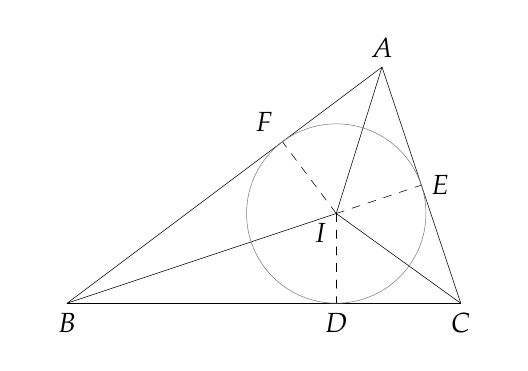
\begin{tikzpicture}
                \tkzInit[xmin=-0.5,xmax=5.5,ymin=-0.5,ymax=3.5]
                \tkzClip
                \tkzDefPoint(4,3){A}
                \tkzDefPoint(0,0){B}
                \tkzDefPoint(5,0){C}
                \tkzLabelPoints[above](A)
                \tkzLabelPoints[below](B)
                \tkzLabelPoints[below](C)
                \tkzDrawSegments(A,B B,C C,A)
            
                \tkzDefCircle[in](A,B,C)
                \tkzGetPoint{I}
                \tkzLabelPoints[below left](I)
            
                \tkzDrawSegments(A,I);
                \tkzDrawSegments(B,I);
                \tkzDrawSegments(C,I);
            
                \tkzDefLine[orthogonal=through I](A,B)
                \tkzGetPoint{r1}
                \tkzInterLL(I,r1)(A,B)
                \tkzGetPoint{F}

                \tkzDefLine[orthogonal=through I](B,C)
                \tkzGetPoint{r2}
                \tkzInterLL(I,r2)(B,C)
                \tkzGetPoint{D}

                \tkzDefLine[orthogonal=through I](C,A)
                \tkzGetPoint{r3}
                \tkzInterLL(I,r3)(C,A)
                \tkzGetPoint{E}

                \tkzDrawSegments[dashed](I,D)
                \tkzDrawSegments[dashed](I,E)
                \tkzDrawSegments[dashed](I,F)

                \tkzDrawCircle(I,F)

                \tkzLabelPoints[below](D);
                \tkzLabelPoints[right](E);
                \tkzLabelPoints[above left](F);
            \end{tikzpicture}
            \caption{三角形正切半角公式示意图}
        \end{center}
    \end{figure}
    
\newpage

    由上述推导结论可得:
    \begin{align}
        EA=p-a
    \end{align}\\
    由直角三角形$\triangle AEI$可得:
    \begin{align}
        \tan{\frac{A}{2}}
        &=\frac{EI}{EA}\\[3mm]
        &=\frac{r}{p-a}\\[3mm]
        &=\frac{r\cdot p}{p\cdot(p-a)}\\[3mm]
        &=\frac{S_{\triangle}}{p\cdot(p-a)}
    \end{align}\\
    由公式$09$代入后可得:
    \begin{align}
        \tan{\frac{A}{2}}
        &=\frac{\sqrt{p\cdot(p-a)\cdot(p-b)\cdot(p-c)}}{p\cdot(p-a)}\\[3mm]
        &=\sqrt{\frac{p\cdot(p-a)\cdot(p-b)\cdot(p-c)}{p^2\cdot(p-a)^2}}\\[3mm]
        &=\sqrt{\frac{(p-b)\cdot(p-c)}{p\cdot(p-a)}}
    \end{align}

\newpage

\subsubsection{三角形的正弦半角公式}
    三角形的正弦半角公式:
    \begin{large}
        \begin{align*}
            \sin{\frac{A}{2}}=\sqrt{\frac{(p-b)\cdot(p-c)}{b\cdot c}}\\[3mm]
            \sin{\frac{B}{2}}=\sqrt{\frac{(p-c)\cdot(p-a)}{c\cdot a}}\\[3mm]
            \sin{\frac{C}{2}}=\sqrt{\frac{(p-a)\cdot(p-b)}{a\cdot b}}
        \end{align*}
    \end{large}\\
    根据三角形的正切半角公式可得:
    \setcounter{equation}{0}
    \begin{align}
        \cot{\frac{A}{2}}=\sqrt{\frac{p\cdot(p-a)}{(p-b)\cdot(p-c)}}
    \end{align}\\
    由三角比的平方关系开始推导:\vspace{5pt}
    \begin{align}
        &\csc^2{\frac{A}{2}}-\cot^2{\frac{A}{2}}=1\\[3mm]
        &\csc^2{\frac{A}{2}}=1+\cot^2{\frac{A}{2}}\\[3mm]
        &\csc^2{\frac{A}{2}}=1+\frac{p\cdot(p-a)}{(p-b)\cdot(p-c)}\\[3mm]
        &\csc^2{\frac{A}{2}}=\frac{p\cdot(p-a)+(p-b)\cdot(p-c)}{(p-b)\cdot(p-c)}\\[3mm]
        &\csc^2{\frac{A}{2}}=\frac{p\cdot(p+b+c-2p)+(p-b)\cdot(p-c)}{(p-b)\cdot(p-c)}\\[3mm]
        &\csc^2{\frac{A}{2}}=\frac{p^2+pb+pc-2p^2+p^2-pb-pc+bc}{(p-b)\cdot(p-c)}\\[3mm]
        &\csc^2{\frac{A}{2}}=\frac{b\cdot c}{(p-b)\cdot(p-c)}\\[3mm]
        &\sin^2{\frac{A}{2}}=\frac{(p-b)\cdot(p-c)}{b\cdot c}\\[3mm]
        &\sin{\frac{A}{2}}=\sqrt{\frac{(p-b)\cdot(p-c)}{b\cdot c}}
    \end{align}

\newpage

\subsubsection{三角形的余弦半角公式}
    三角形的余弦半角公式:
    \begin{large}
        \begin{align*}
            \cos{\frac{A}{2}}=\sqrt{\frac{p\cdot(p-a)}{b\cdot c}}\\[3mm]
            \cos{\frac{B}{2}}=\sqrt{\frac{p\cdot(p-b)}{c\cdot a}}\\[3mm]
            \cos{\frac{C}{2}}=\sqrt{\frac{p\cdot(p-c)}{a\cdot b}}\\[3mm]
        \end{align*}
    \end{large}
    根据三角形的正切半角公式可得:
    \setcounter{equation}{0}
    \begin{align}
        \tan{\frac{A}{2}}=\sqrt{\frac{(p-b)\cdot(p-c)}{p\cdot(p-a)}}
    \end{align}\\
    由三角比的平方关系开始推导:
    \begin{align}
        &\sec^2{\frac{A}{2}}-\tan^2{\frac{A}{2}}=1\\[3mm]
        &\sec^2{\frac{A}{2}}=1+\tan^2{\frac{A}{2}}\\[3mm]
        &\sec^2{\frac{A}{2}}=1+\frac{(p-b)\cdot(p-c)}{p\cdot(p-a)}\\[3mm]
        &\sec^2{\frac{A}{2}}=\frac{p\cdot(p-a)+(p-b)\cdot(p-c)}{p\cdot(p-a)}\\[3mm]
        &\sec^2{\frac{A}{2}}=\frac{p\cdot(p+b+c-2p)+(p-b)\cdot(p-c)}{p\cdot(p-a)}\\[3mm]
        &\sec^2{\frac{A}{2}}=\frac{p^2+pb+pc-2p^2+p^2-pb-pc+bc}{p\cdot(p-a)}\\[3mm]
        &\sec^2{\frac{A}{2}}=\frac{b\cdot c}{p\cdot(p-a)}\\[3mm]
        &\cos^2{\frac{A}{2}}=\frac{p\cdot(p-a)}{b\cdot c}\\[3mm]
        &\cos{\frac{A}{2}}=\sqrt{\frac{p\cdot(p-a)}{b\cdot c}}
    \end{align}

\newpage

\subsection{三角形的第二组面积公式}
    本章将研究三角形中与半角的三角函数相关的面积公式,并进行相应推导。

\subsubsection{三角形面积公式$16$}
    三角形面积公式$16$:
    \begin{large}
        \begin{align*}
            &S_{\triangle}=p\cdot(p-a)\cdot\tan{\frac{A}{2}}\\[3mm]
            &S_{\triangle}=p\cdot(p-b)\cdot\tan{\frac{B}{2}}\\[3mm]
            &S_{\triangle}=p\cdot(p-c)\cdot\tan{\frac{C}{2}}
        \end{align*}
    \end{large}\\
    将三角形正切半角公式推导的中间步骤变形可得:\vspace{5pt}
    \setcounter{equation}{0}
    \begin{align}
        &\tan{\frac{A}{2}}=\frac{S_{\triangle}}{p\cdot(p-a)}\\[3mm]
        &S_{\triangle}=p\cdot(p-a)\cdot\tan{\frac{A}{2}}
    \end{align}

\subsubsection{三角形面积公式$17$}
    三角形面积公式$17$:
    \begin{large}
        \begin{equation*}
            S_{\triangle}=p^2\cdot\tan{\frac{A}{2}}\cdot\tan{\frac{B}{2}}\cdot\tan{\frac{C}{2}}
        \end{equation*}
    \end{large}\\
    由公式$16$可以得到:\vspace{5pt}
    \setcounter{equation}{0}
    \begin{align}
        &\tan{\frac{A}{2}}\cdot\tan{\frac{B}{2}}\cdot\tan{\frac{C}{2}}=\frac{S_{\triangle}}{p\cdot(p-a)}\cdot\frac{S_{\triangle}}{p\cdot(p-b)}\frac{S_{\triangle}}{p\cdot(p-c)}\\[3mm]
        &\tan{\frac{A}{2}}\cdot\tan{\frac{B}{2}}\cdot\tan{\frac{C}{2}}=\frac{S_{\triangle}~^3}{p^3\cdot(p-a)\cdot(p-b)\cdot(p-c)}\\[3mm]
        &\tan{\frac{A}{2}}\cdot\tan{\frac{B}{2}}\cdot\tan{\frac{C}{2}}=\frac{S_{\triangle}~^2}{p\cdot(p-a)\cdot(p-b)\cdot(p-c)}\cdot\frac{S_{\triangle}}{p^2}\\[3mm]
        &\tan{\frac{A}{2}}\cdot\tan{\frac{B}{2}}\cdot\tan{\frac{C}{2}}=\frac{S_{\triangle}~^2}{S_{\triangle}~^2}\cdot\frac{S_{\triangle}}{p^2}\\[3mm]
        &\tan{\frac{A}{2}}\cdot\tan{\frac{B}{2}}\cdot\tan{\frac{C}{2}}=\frac{S_{\triangle}}{p^2}\\[3mm]
        &~S_{\triangle}=p^2\cdot\tan{\frac{A}{2}}\cdot\tan{\frac{B}{2}}\cdot\tan{\frac{C}{2}}
    \end{align}

\newpage

\subsubsection{三角形面积公式$18$}
    三角形面积公式$18$:
    \begin{large}
        \begin{equation*}
            S_{\triangle}=a\cdot b\cdot c\cdot \frac{1}{p}\cdot\cos{\frac{A}{2}}\cdot\cos{\frac{B}{2}}\cdot\cos{\frac{C}{2}}
        \end{equation*}
    \end{large}\\
    由三角形余弦半角公式可以得到:\vspace{5pt}
    \setcounter{equation}{0}
    \begin{align}
        &\cos^2{\frac{A}{2}}\cdot\cos^2{\frac{B}{2}}\cdot\cos^2{\frac{C}{2}}=\frac{p\cdot(p-a)}{b\cdot c}\cdot\frac{p\cdot(p-b)}{c\cdot a}\cdot\frac{p\cdot(p-c)}{a\cdot b}\\[3mm]
        &\cos^2{\frac{A}{2}}\cdot\cos^2{\frac{B}{2}}\cdot\cos^2{\frac{C}{2}}=\frac{p^3\cdot(p-a)\cdot(p-b)\cdot(p-c)}{a^2\cdot b^2\cdot c^2}\\[3mm]
        &\cos^2{\frac{A}{2}}\cdot\cos^2{\frac{B}{2}}\cdot\cos^2{\frac{C}{2}}=\frac{p^2\cdot S_{\triangle}~^2}{a^2\cdot b^2\cdot c^2}\\[3mm]
        &\cos{\frac{A}{2}}\cdot\cos{\frac{B}{2}}\cdot\cos{\frac{C}{2}}=\frac{p\cdot S_{\triangle}}{a\cdot b\cdot c}\\[3mm]
        &~S_{\triangle}=a\cdot b\cdot c\cdot \frac{1}{p}\cdot\cos{\frac{A}{2}}\cdot\cos{\frac{B}{2}}\cdot\cos{\frac{C}{2}}
    \end{align}\\

\subsubsection{三角形面积公式$19$}
    三角形面积公式$19$:
    \begin{large}
        \begin{equation*}
            S_{\triangle}~^2=a\cdot b\cdot c\cdot p\cdot\sin{\frac{A}{2}}\cdot\sin{\frac{B}{2}}\cdot\sin{\frac{C}{2}}
        \end{equation*}
    \end{large}\\
    由三角形正弦半角公式可以得到:\vspace{5pt}
    \setcounter{equation}{0}
    \begin{align}
        &\sin^2{\frac{A}{2}}\cdot\sin^2{\frac{B}{2}}\cdot\sin^2{\frac{C}{2}}=\frac{(p-b)\cdot(p-c)}{b\cdot c}\cdot\frac{(p-c)\cdot(p-a)}{c\cdot a}\cdot\frac{(p-a)\cdot(p-b)}{a\cdot b}\\[3mm]
        &\sin^2{\frac{A}{2}}\cdot\sin^2{\frac{B}{2}}\cdot\sin^2{\frac{C}{2}}=\frac{p^2\cdot(p-a)^2\cdot(p-b)^2\cdot(p-c)^2}{a^2\cdot b^2\cdot c^2\cdot p^2}\\[3mm]
        &\sin^2{\frac{A}{2}}\cdot\sin^2{\frac{B}{2}}\cdot\sin^2{\frac{C}{2}}=\frac{S_{\triangle}~^4}{a^2\cdot b^2\cdot c^2\cdot p^2}\\[3mm]
        &\sin{\frac{A}{2}}\cdot\sin{\frac{B}{2}}\cdot\sin{\frac{C}{2}}=\frac{S_{\triangle}}{a\cdot b\cdot c}\\[3mm]
        &~S_{\triangle}~^2=a\cdot b\cdot c\cdot p\cdot\sin{\frac{A}{2}}\cdot\sin{\frac{B}{2}}\cdot\sin{\frac{C}{2}}
    \end{align}

\newpage

\subsubsection{三角形面积公式$20$}
    三角形面积公式$20$:
    \begin{large}
        \begin{equation*}
            S_{\triangle}=4\cdot R\cdot p\cdot\sin{\frac{A}{2}}\cdot\sin{\frac{B}{2}}\cdot\sin{\frac{C}{2}}
        \end{equation*}
    \end{large}\\
    将公式$04$代入公式$19$:
    \setcounter{equation}{0}
    \begin{align}
        &S_{\triangle}~^2=a\cdot b\cdot c\cdot p\cdot\sin{\frac{A}{2}}\cdot\sin{\frac{B}{2}}\cdot\sin{\frac{C}{2}}\\[3mm]
        &S_{\triangle}\cdot\frac{a\cdot b\cdot c}{4R}=a\cdot b\cdot c\cdot p\cdot\sin{\frac{A}{2}}\cdot\sin{\frac{B}{2}}\cdot\sin{\frac{C}{2}}\\[3mm]
        &S_{\triangle}=4\cdot R\cdot p\cdot\sin{\frac{A}{2}}\cdot\sin{\frac{B}{2}}\cdot\sin{\frac{C}{2}}
    \end{align}\\

\subsubsection{三角形面积公式$21$}
    三角形面积公式$21$:
    \begin{large}
        \begin{equation*}
            S_{\triangle}=4\cdot R\cdot r\cdot\cos{\frac{A}{2}}\cdot\cos{\frac{B}{2}}\cdot\cos{\frac{C}{2}}
        \end{equation*}
    \end{large}\\
    将公式$04$代入公式$18$:
    \setcounter{equation}{0}
    \begin{align}
        &S_{\triangle}=a\cdot b\cdot c\cdot \frac{1}{p}\cdot\cos{\frac{A}{2}}\cdot\cos{\frac{B}{2}}\cdot\cos{\frac{C}{2}}\\[3mm]
        &\frac{a\cdot b\cdot c}{4R}=a\cdot b\cdot c\cdot \frac{1}{p}\cdot\cos{\frac{A}{2}}\cdot\cos{\frac{B}{2}}\cdot\cos{\frac{C}{2}}\\[3mm]
        &p=4\cdot R\cdot\cos{\frac{A}{2}}\cdot\cos{\frac{B}{2}}\cdot\cos{\frac{C}{2}}
    \end{align}\\
    将上述结论代入公式$05$:
    \begin{align}
        &S_{\triangle}=r\cdot p\\[3mm]
        &S_{\triangle}=r\cdot 4\cdot R\cdot\cos{\frac{A}{2}}\cdot\cos{\frac{B}{2}}\cdot\cos{\frac{C}{2}}\\[3mm]
        &S_{\triangle}=4\cdot R\cdot r\cdot\cos{\frac{A}{2}}\cdot\cos{\frac{B}{2}}\cdot\cos{\frac{C}{2}}
    \end{align}

\newpage

\subsubsection{三角形面积公式$22$}
    三角形面积公式$22$:
    \begin{large}
        \begin{equation*}
            S_{\triangle}=r^2\cdot\cot{\frac{A}{2}}\cdot\cot{\frac{B}{2}}\cdot\cot{\frac{C}{2}}
        \end{equation*}
    \end{large}\\
    将公式$05$和公式$17$对比:
    \setcounter{equation}{0}
    \begin{align}
        &S_{\triangle}=r\cdot p\\[3mm]
        &S_{\triangle}=p^2\cdot\tan{\frac{A}{2}}\cdot\tan{\frac{B}{2}}\cdot\tan{\frac{C}{2}}\\[3mm]
        &r=p\cdot\tan{\frac{A}{2}}\cdot\tan{\frac{B}{2}}\cdot\tan{\frac{C}{2}}\\[3mm]
        &p=\frac{r}{\tan{\dfrac{A}{2}}\cdot\tan{\dfrac{B}{2}}\cdot\tan{\dfrac{C}{2}}}
    \end{align}\\
    将上述结论代入公式$17$:\vspace{5pt}
    \begin{align}
        &S_{\triangle}=p^2\cdot\tan{\frac{A}{2}}\cdot\tan{\frac{B}{2}}\cdot\tan{\frac{C}{2}}\\[3mm]
        &S_{\triangle}=\frac{r^2}{\tan^2{\dfrac{A}{2}}\cdot\tan^2{\dfrac{B}{2}}\cdot\tan^2{\dfrac{C}{2}}}\cdot\tan{\frac{A}{2}}\cdot\tan{\frac{B}{2}}\cdot\tan{\frac{C}{2}}\\[3mm]
        &S_{\triangle}=\frac{r^2}{\tan{\dfrac{A}{2}}\cdot\tan{\dfrac{B}{2}}\cdot\tan{\dfrac{C}{2}}}\\[3mm]
        &S_{\triangle}=r^2\cdot\cot{\frac{A}{2}}\cdot\cot{\frac{B}{2}}\cdot\cot{\frac{C}{2}}
    \end{align}

    

\end{document}
